\documentclass[12pt,letterpaper,twoside]{article}
\usepackage{../cme211}
\usepackage{algorithm2e}

\def\D{\mathrm{d}}

\begin{document}
\title{Lecture 9: \LaTeX \vspace{-5ex}}
\date{Fall 2020}
\maketitle

% {\footnotesize
% \paragraph{Topics Introduced:} \LaTeX.
% }
% \vspace{-3ex}
\vspace{-6ex}
\section{History}
\vspace{-2.5ex}
% I'm personally a huge fan of \TeX.\footnote{Anecdotally, I learned how
% to use it over a weekend when writing my baccalaureate thesis. I felt
% that the mathematical symbols in Word limited my ability to express my
% ideas, and that having tables bleed across pages distracted away from
% key results. Although it has a learning curve, it's an industry
% standard across STEM fields that's not going away.}
\subsection{\TeX}
% \paragraph{Knuth: Author of ``Art of Programming'', and \TeX}
\TeX was primarily authored by
\href{https://en.wikipedia.org/wiki/Donald_Knuth}{Donald
  Knuth}. Donald started writing
\href{https://en.wikipedia.org/wiki/The_Art_of_Computer_Programming}{The
  Art of Computer Programming} back in 1962, which is a volume of
programming algorithms and analyses which is still being
worked on today. In the 70's, one of the volumes had to be typeset all
over again because an industry standard was moving away from
\href{https://en.wikipedia.org/wiki/Hot_metal_typesetting}{mechanical
  typesetting} (pressing ink onto paper using metal molds of
characters) and toward
\href{https://en.wikipedia.org/wiki/Phototypesetting}{phototypesetting}
(projecting light through a film-negative of a character onto
\href{https://en.wikipedia.org/wiki/Photographic_paper}{photographic
  paper}
in a light-proof canister).

\paragraph{Motivation for \TeX}
Donald was frustrated by this, and
separately but around this same time, he was impressed with having
seen for the first time a digital
typesetting system. In 1977, he outlined the basic features of \TeX
and planned to finish it over a sabattical in
1978. The name comes from combining a sequence of mathematical
characters Tau, Epsilon, and Chi.
The program has undergone several major changes, including
rewriting it entirely in \TeX '82 to make it a
\href{https://en.wikipedia.org/wiki/Turing_completeness}{Turing
  Complete} language, which means that the language can be used to
simulate \emph{any} computational aspects of any other computer
(language).

\paragraph{Stability of \TeX}
The language \TeX is now quite stable. It uses an idiosyncratic
version numbering system in which updates are signified by adding an
additional digit to the end of the current version number, in a way
such that the version numbers asymptotically approach $\pi$. It's
currently in version 3.14159265, and this was updated in January
2014. The design was frozen after version 3 to reflect that no new
features will be added, only bugs will be fixed. Even though he's
proposed additional feature enhancements, Knuth believes the value in a
stable typesetting system outweights further improvements. The final
version of \TeX will be released after Knuth passes, at which point
the version number will be changed to $\pi$ exactly and all bugs will
become features. See: \href{http://www.ntg.nl/maps/05/34.pdf}{``The
  Future of \TeX and METAFONT'' (Knuth '90)}.

\paragraph{Bugs and Monetary Awards}
Donald
Knuth has maintained a detailed listing of all bugs ever found (and of course
corrected) in \TeX since 1982. There are currently just over 400
listings. Knuth offers
\href{https://en.wikipedia.org/wiki/TeX#Development}{monetary awards}
to individuals who find bugs,
starting at one hexadecimal dollar (\$2.56) and doubling every year
until frozen at its current value of \$327.68. Anecdotally, Knuth hasn't
lost much money in this endeavor since recipients of these checks
enjoy framing them on their walls instead of cashing them.

\subsection{\LaTeX} Leslie Lamport authored an extension of \TeX in
the early 80's. It builds off of \TeX in a way that is designed to be
easier for writers. Essentially,
\href{https://en.wikipedia.org/wiki/LaTeX}{\LaTeX}
can be coarsely described as a collection of \TeX \, macros
(e.g. for making chapters, section headers, subsections, etc.). Its
current version is $\textrm{\LaTeX} 2_{\epsilon}$. It is still under active
development, and is less stable than \TeX. There is a research version
of
\href{https://www.latex-project.org/help/documentation/ltx3info.pdf}{\LaTeX
  3}
being developed. Here is a link to an
\href{http://texdoc.net/texmf-dist/doc/latex/latex2e-help-texinfo/latex2e.pdf}{unofficial reference}.

\paragraph{Markup Languages}
A \href{https://en.wikipedia.org/wiki/Markup_language#Etymology}{\emph{markup
  language}} lets us syntatically differentiate between
formatting modifiers and content. The name comes from when skilled
typographers would ``mark up'' manuscripts by hand, annotating in the
margins what typeface style, font, and size should be applied to each
part of the document; after the manuscript was marked up by hand, it
would be passed off for actual typesetting. Markup languages are in
contrast with \href{https://en.wikipedia.org/wiki/WYSIWYG}{What
You See Is What You Get} programs, e.g. Microsoft Word, which allows
the writer to see the end product as they are prototyping.

\paragraph{Relating LaTeX and HTML}
\LaTeX \, is a document markup language, and is targeted toward high
quality print documents, appearing in scientific or academic journals.
\href{https://en.wikipedia.org/wiki/HTML}{HTML}
is also a document markup language, which targets web browsers. The
\emph{elements} of HTML are \href{https://en.wikipedia.org/wiki/HTML#Elements}{\emph{tags}}.
\TeX \, commands are also now used to typeset equations on the web, and
so even if you don't wish to live in \LaTeX, they're still worth
learning. E.g. markdown languages support some \TeX \, commands.

\begin{figure}[h]
\centering
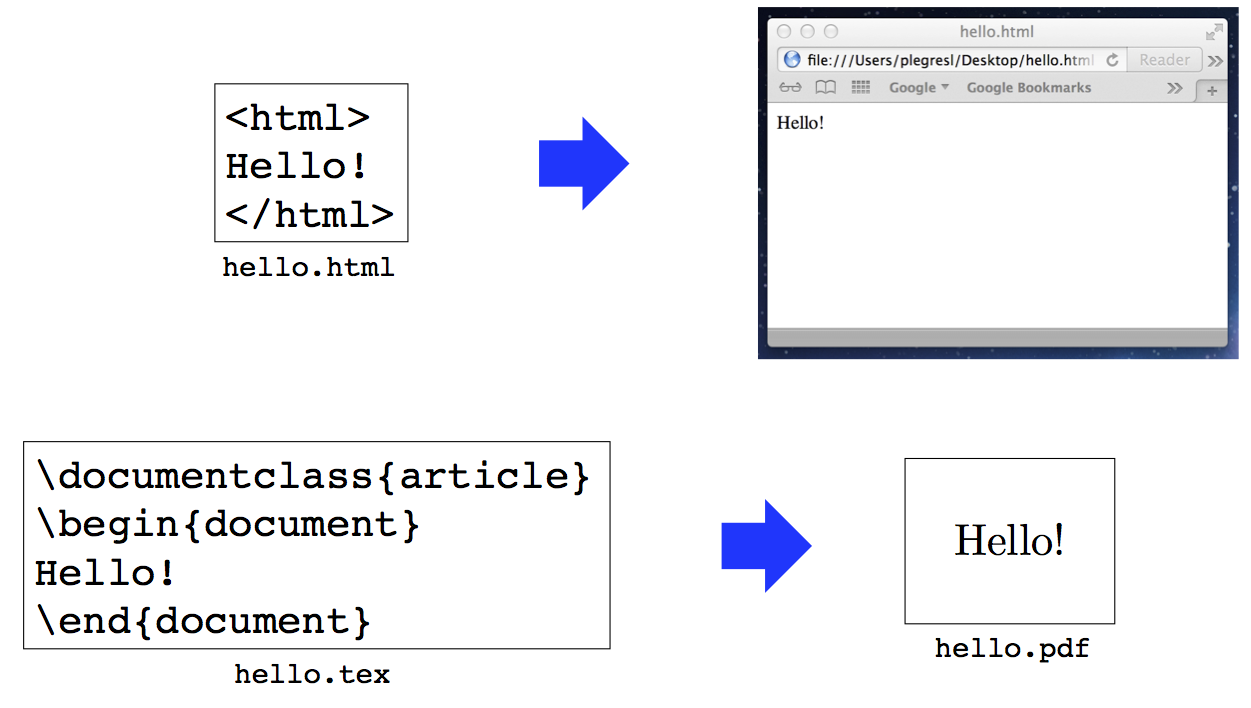
\includegraphics[scale=0.65]{fig/markup.png}
\caption{\footnotesize We show raw source code used to generate a simple HTML
  document and correspondingly for a \LaTeX document. In either case,
  we must delimit our body of text in some way, either by
  \texttt{<html>} and \texttt{</html>} or \texttt{$\backslash$begin\{document\}}
    and \texttt{$\backslash$end\{document\}}.} 
\end{figure}

\section{Setup and Usage}

\subsection{Installation}
We provide different recommendations based on the operating system.
{
  \small
\begin{itemize}
\item
  Windows: \url{http://miktex.org/about}
\item
  Mac OSX: \url{https://tug.org/mactex/}
\item
  Ubuntu: \texttt{\$\ sudo\ apt-get\ install\ texlive}
\item
  Fedora: \texttt{\$\ sudo\ yum\ install\ texlive-scheme-medium}
\end{itemize}
}

Note: on Linux distributions, you may have to install other
\texttt{texlive} packages to get the full TeXLive distribution. Ubuntu
has the package \texttt{texlive-full}. Fedora has the package collection
\texttt{texlive-scheme-full}. These are large downloads. Be prepared to
wait. Don't install TeX at the last moment!

\subsection{Compiling a \texttt{.tex} file into a PDF} We write our
\LaTeX \, markup in \texttt{.tex} files, similar to how we write Python code in
\texttt{.py} files. When we want to compile the source code into a
PDF, we need to use a separate program, e.g. \texttt{pdflatex}.\footnote{
TeXLive is already installed on \texttt{rice.stanford.edu}, and this
includes \texttt{pdflatex}. The primary access
point for CME 211 will be the command line program \texttt{pdflatex}.}
In general, we compile a \texttt{.tex} document into a \texttt{.pdf}
file via the following.
\begin{verbatim}
$ pdflatex myfile.tex    # myfile.pdf is produced.
\end{verbatim}
We can even use a GNU
\href{https://en.wikipedia.org/wiki/Makefile}{makefile}
to drive \TeX.

\paragraph{Emacs and Vim} Recall our extensible editors? Emacs supports
\href{https://www.emacswiki.org/emacs/AUCTeX}{AUC-TeX}, which easily
allows us to compile LaTeX into a pdf without ever having to leave our
editor. We just use the key-strokes \texttt{C-c C-c}. Here's
\href{https://vigou3.gitlab.io/emacs-modified-macos/}{an installation
  of Emacs} (complete with AUCTeX, and other goodies like \href{https://ess.r-project.org/}{ESS}). Note
that installing emacs is totally separate from installing
\TeX. Similarly for Vim, there is
\href{http://vim-latex.sourceforge.net/}{\texttt{Vim-LaTeX}}.

\paragraph{GUIs} Of course, some may enjoy a graphical
interface. Options include TeXShop, TeXWorks, and TeXMaker.\footnote{Note that there are also programs like \href{https://www.overleaf.com/}{Overleaf}, an online tool
for writing \TeX documents, compiling, and sharing with others; you
can get a temporary educational account with free access, but
again they're happy to
\href{https://www.overleaf.com/user/subscription/plans}{charge you
  \$15/month} thereafter. They advertise features like being able to Sync with Dropbox and
Github, and provide full tracking history. Do these features sound familiar to
other free tools that we've learned how to use, like Git?}


\subsection{Hello world}
See: \texttt{tex/hello.tex}:

{\small
\begin{verbatim}
\documentclass{article}
\begin{document}
Hello
\end{document}
\end{verbatim}
}

Typesetting instructions (from the same directory as the lecture notes
are contained in):

\begin{verbatim}
$ cd tex
$ pdflatex hello.tex
\end{verbatim}

This creates \texttt{hello.pdf}. To be explicit, for our class, and if
we wanted to use Emacs on Rice (which is already installed with AUCTeX)
\begin{verbatim}
ssh <sunetid>@rice.stanford.edu
# Login and Navigate to your favorite working directory.
emacs hello.tex
# Create file just as above. Execute: C-c C-c. This  compiles a pdf.
\end{verbatim}
Then, one could go to \url{https://afs.stanford.edu/} to view the pdf
document that was created on \texttt{rice}. If we wanted to perform
the entire process locally, we could
install LaTeX on our machine and forego having to \texttt{ssh}
into \texttt{rice} and then fetch our \texttt{.pdf} via an online
browser (or perhaps \texttt{scp}).

\section{Overview of LaTeX}
There's a lot of formatting options in LaTeX, and it can feel
overwhelming at first.
\vspace{-2ex}
\subsection{Document Formatting}
\subsubsection{Document Class - Specifying Page Layout}
A
\href{https://en.wikibooks.org/wiki/LaTeX/Document_Structure\#Document_classes}{document
  class} defines the layout for a page. Options include:

{
  \small
\begin{itemize}
\item
  \texttt{article} - general purpose class for publications, short reports,   etc.
\item
  \texttt{proc} - proceedings (based on the article class)
\item
  \texttt{report} - for longer reports with several chapters, small
  books, and theses.
\item
  \texttt{book} - for real books.
\item
  \texttt{slides} - for presentation slides. See as well: \href{https://en.wikibooks.org/wiki/LaTeX/Presentations\#The_Beamer_package}{beamer}.
\item
  \texttt{letter} - writing letters.
\end{itemize}
}

For each of these classes, there are options that can be
applied. E.g. we can choose the font, the paper size,
whether to use one or two columns, one or two-sided
outputs, landscape mode, etc.

\paragraph{Custom Classes} A class can be defined using a
\texttt{.cls} file. Various organizations will
also distribute customized document classes
for various purposes. These can be useful if you plan to submit your
work to a particular vendor or publisher. E.g.

\begin{itemize}
\item
  SIAM LaTeX: \url{https://www.siam.org/journals/auth-info.php}.
\item
  Stanford PhD thesis template:
  \newline
  \url{https://library.stanford.edu/research/bibliography-management/latex-and-bibtex}.
\end{itemize}

\subsection{Introduction to Custom Formatting}
\subsubsection{White space}

White space is normalized so \texttt{1} to \texttt{n} spaces are treated
the same.

\begin{figure}[h]
\centering
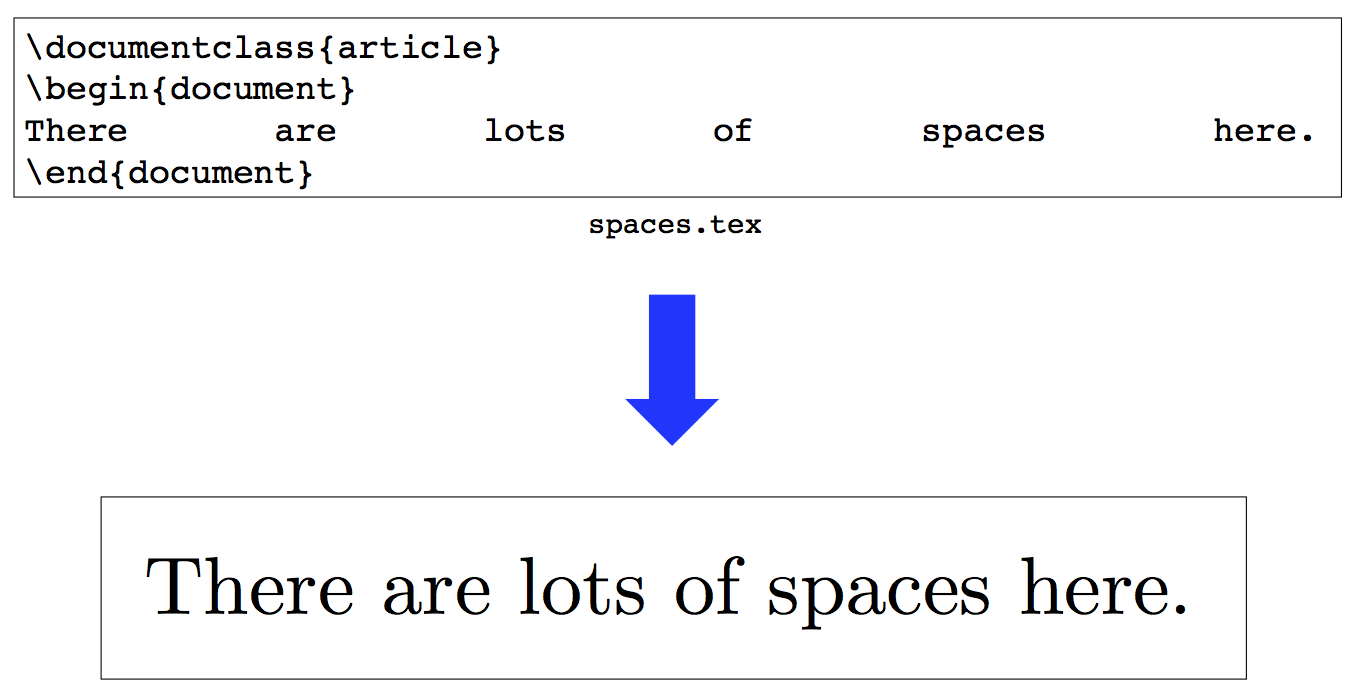
\includegraphics[scale=0.45]{fig/spaces.png}
\caption{The space operator acts the same whether used once or consecutively.}
\end{figure}

If you want to add \emph{additional} spacing, there's many different
ways to do this. You could, for example, use either \texttt{\,} to
indicate additional separation, or you could use
\href{http://www.emerson.emory.edu/services/latex/latex_142.html}{\texttt{$\backslash$hspace\{length\}}}, where \texttt{length} is an argument such as
inches, millimeters, or points. E.g. \texttt{$\backslash$hspace\{2pt\}}, or \texttt{$\backslash$hspace\{1cm\}} are valid.

\subsubsection{Paragraphs}
Paragraphs are delimited by multiple line breaks.
\begin{figure}[h]
\centering
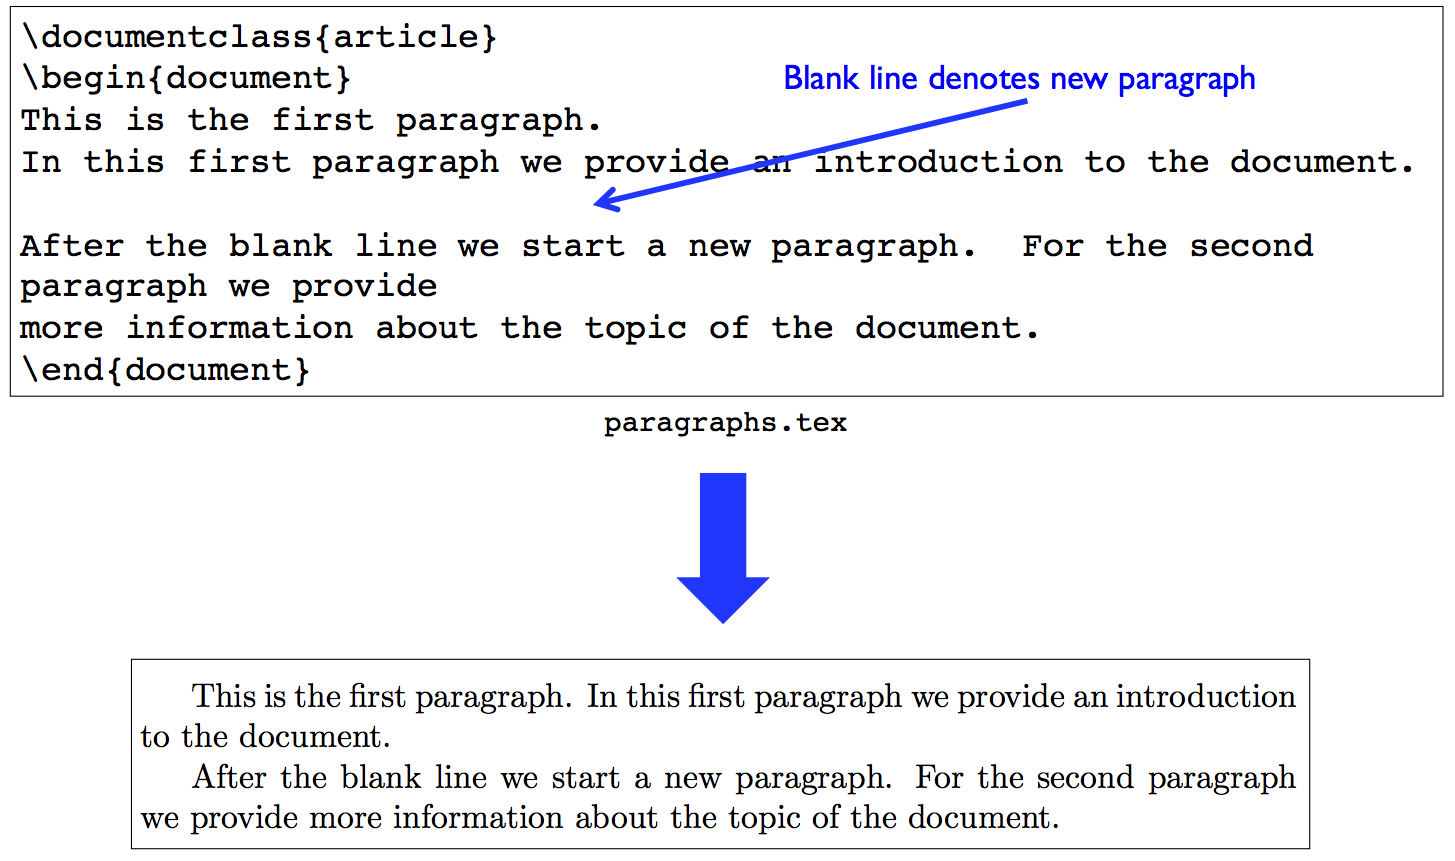
\includegraphics[scale=0.5]{fig/paragraphs.png}
\caption{Multiple line breaks are required in order to indicate a
  paragraph break.}
\end{figure}

\subsubsection{Bulleted list}

We use \texttt{itemize} for lists, which can of
course be nested.

\begin{figure}[h]
\centering
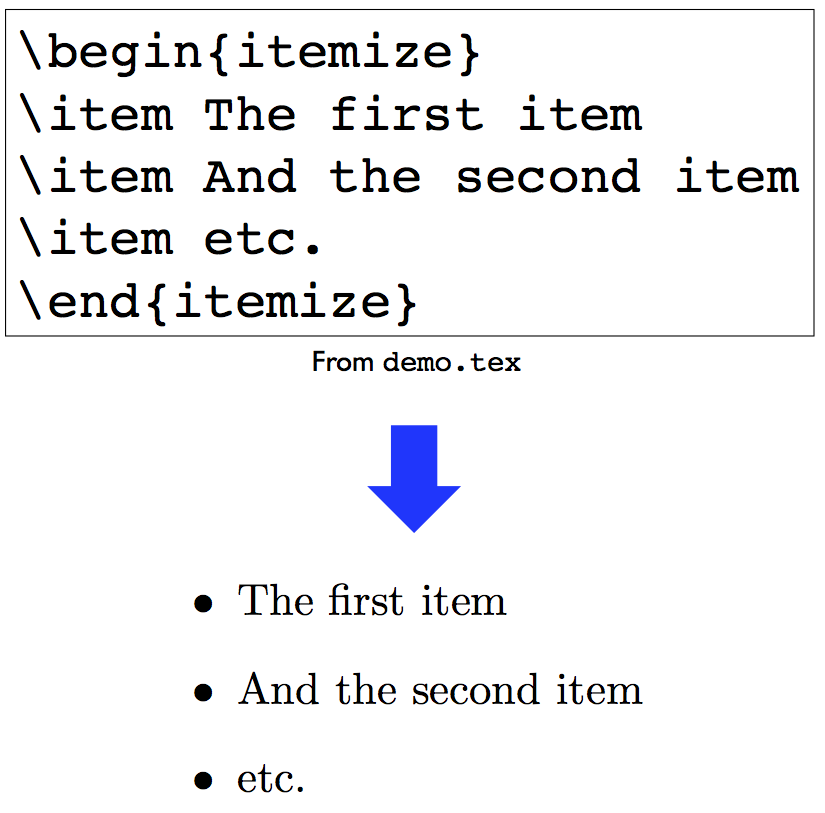
\includegraphics[scale=0.4]{fig/bullets.png}
\caption{Bulleted lists.}
\end{figure}

If we wish for enumerated items, we can simply use
\texttt{$\backslash$begin\{enumerate\}} and
\texttt{$\backslash$end\{enumerate\}} to delimit our
list instead, still using the same syntax to
distinguish elements.

\subsection{Special characters}

There are several reserved characters in LaTeX. These take on a
different meaning from their literal counterparts.

\begin{verbatim}
# $ % ^ & _ { } ~ \
\end{verbatim}

\subsubsection{Comments}

Anything which follows a percent symbol (\%) is treated as part of a
comment, i.e. the text which follows it is not treated as content of
the document.

\begin{figure}[!h]
\centering
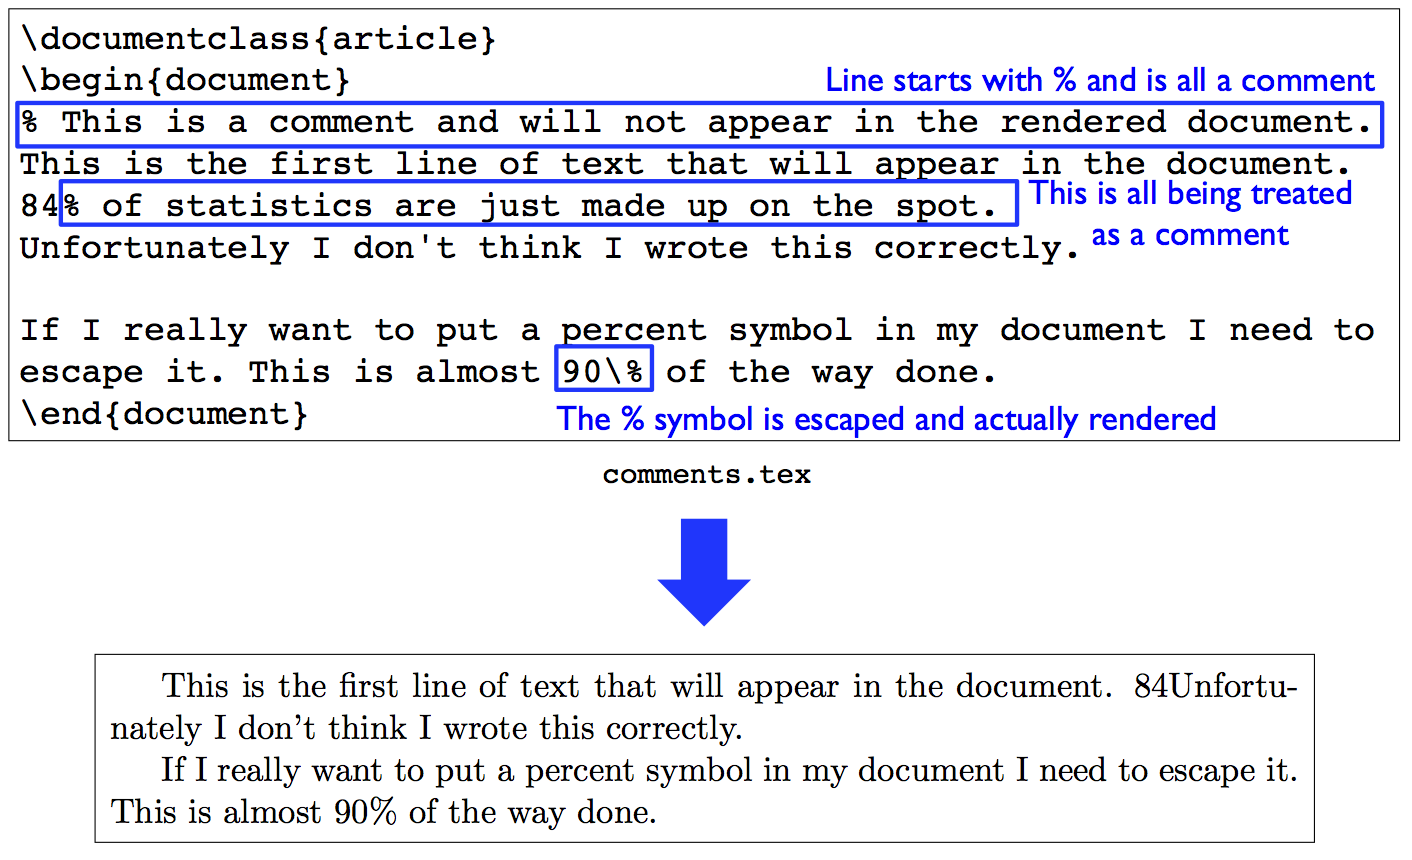
\includegraphics[scale=0.5]{fig/comments.png}
\caption{Comments in LaTeX. Note that anything after the percent symbol (\%) is
  treated as a comment. To treat a special
  character as a literal character, we must escape it using a
  backslash, i.e. \texttt{$\backslash$}.}
\end{figure}

\subsubsection{Groups}

Pairs of curly brackets denote a group and are typically used to limit
the scope of switches:

\begin{figure}[!h]
\centering
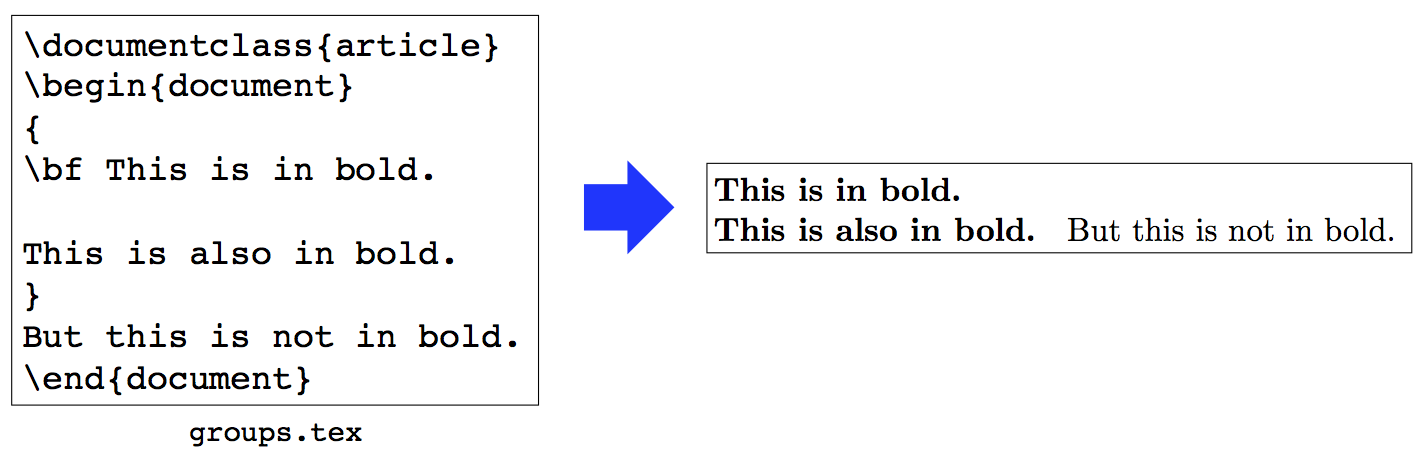
\includegraphics[scale=0.5]{fig/groups.png}
\caption{Groups can be delimited by curly braces.}
\end{figure}

You'll notice above that we used a \emph{command}
to switch to boldface text,
denoted by \texttt{$\backslash$bf}; this is an example of a
\href{https://en.wikibooks.org/wiki/LaTeX/Fonts\#Font_styles}{font style}.

\subsection{Commands}

The general syntax for a \LaTeX \, command is

\begin{verbatim}
\commandname[option1,option2,...]{argument1}{argument2}...
\end{verbatim}

The square brackets delimit optional input arguments, whereas
the curly braces indicate required arguments.

\paragraph{Command Example}
Suppose we want to italicize a selection of text. As opposed to a What
You See Is What You Get, e.g. Microsoft Word where we may highlight a
selection of text and then click the \textbf{bold} icon to display
emboldened text, \LaTeX \, uses a special syntax within the document
to signify that a sequence of characters shall be boldened.

\begin{figure}[h]
\centering
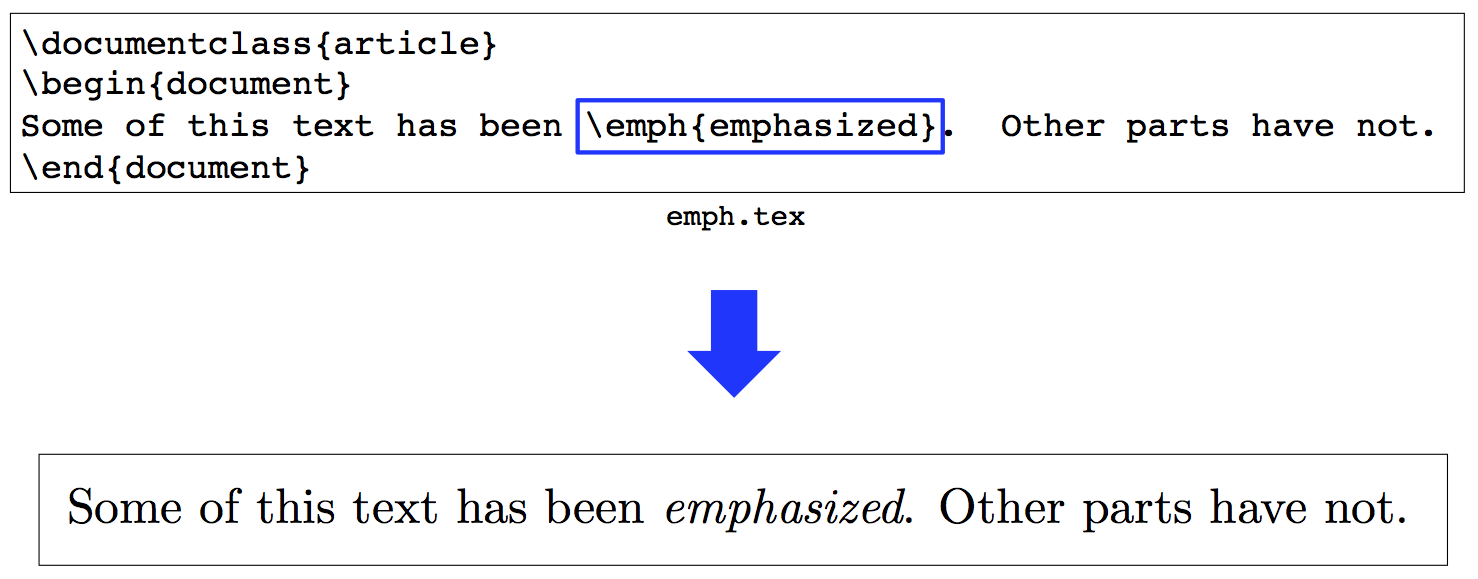
\includegraphics[scale=0.5]{fig/commands.png}
\caption{\footnotesize In the above example, we've used an \texttt{$\backslash$emph}
command to signify that the text contained as input argument should be
italicized.}
\end{figure}

\subsection{Environments}

Environments perform an action on a chunk of text; we can think of an
environment as delimited by two commands.

\begin{verbatim}
\begin{environmentname}
Text to be influenced by this environment
\end{environmentname}
\end{verbatim}

Everything within the environment is treated as an argument to be
acted upon, in a sense. We might ask, why not simply use a single
command with an argument which mimics what would otherwise be the body
of an environment? The answer gets into \href{https://tex.stackexchange.com/a/8382/48589}{technical implementation
details}, but we can think about environments as being more
user-friendly when the argument is intended to be very long, e.g. a
paragraph or an algorithm.

\subsection{Math and Equations in \LaTeX}
Even though we may not have learned yet how to use limits, the below
code should be reasonably easy to interpret, especially alongside the
output.

\begin{figure}[h]
\centering
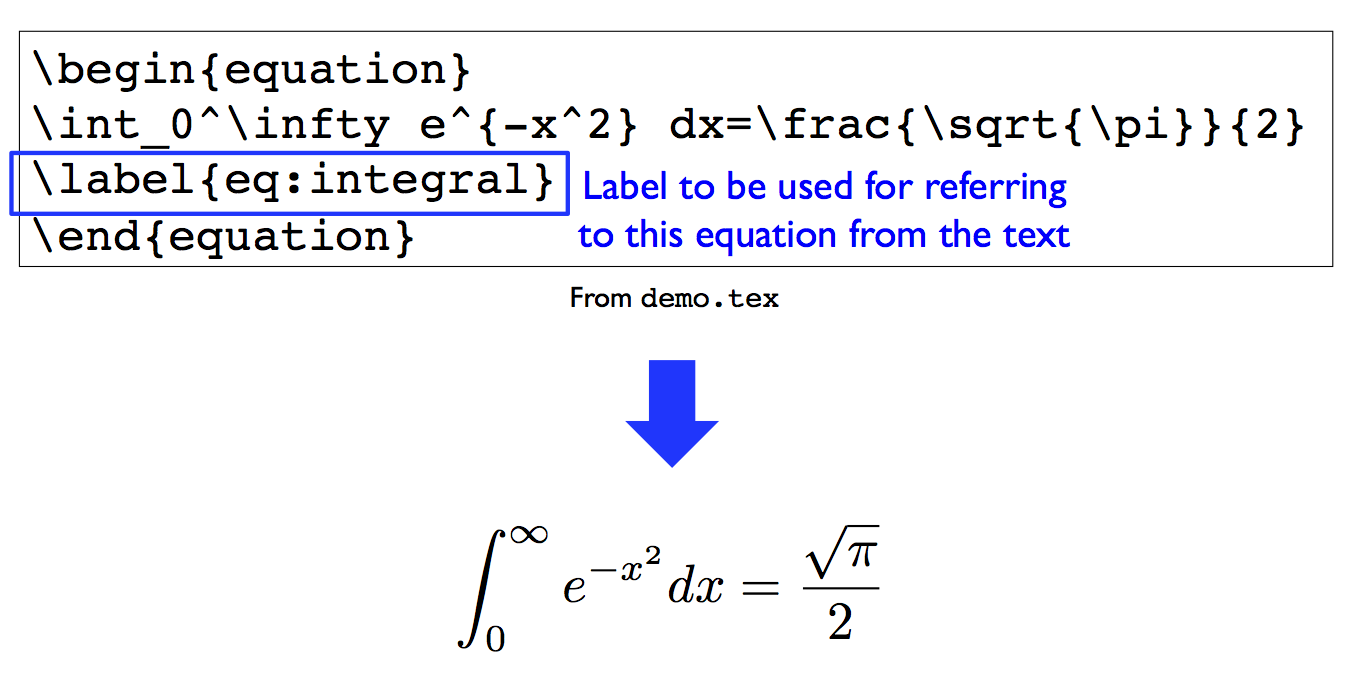
\includegraphics[scale=0.5]{fig/equation.png}
\caption{\footnotesize Out of mathematical curiosity, we remind ourselves of
  \href{https://en.wikipedia.org/wiki/Error_function}{error function}
  and
  \href{https://en.wikipedia.org/wiki/Normal_distribution\#Standard_normal_distribution}{standard
    normals}. The example showcases the use of metacharacters
\texttt{\^} and \texttt{\_} to
provide superscripts and subscripts; notice that we can use them both
concurrently and the result is nicely formatted. The example also
demonstrates that we can nest exponents, or use commands as input
arguments, e.g. $\sqrt{\pi}$.
}
\end{figure}

\paragraph{Operators as Distinguished From Variables}
One small error in this example: operators should appear upright in order to differentiate
themselves from variables. Although this may seem like a nuanced
opinion, it's
\href{https://tex.stackexchange.com/questions/14821/whats-the-proper-way-to-typeset-a-differential-operator}{its
  in fact a standard by ISO 31}.
LaTeX is nice in that it affords us such fine grained
control: to write a differential operator, we can use
\texttt{$\backslash$mathrm\{d\}x} to produce $\D x$.
If we'd like a shorthand, we can
place \texttt{$\backslash$def$\backslash$D\{$\backslash$mathrm\{d\}} in our preamble before the
\texttt{$\backslash$begin\{document\}} in our \texttt{.tex} file,
wherein we have access to a new command anywhere in the body of our
\TeX document, e.g. we can type \texttt{$\backslash$D x} $\leadsto$
$\D x$.

\subsubsection{Personal Favorites for Formatting}
I am fairly particular about formatting
my mathematics, whether it be for a problem set or project proposal: I
want the details to be clear and accessible. A couple tools I find
helpful are: (i) the \texttt{align*} environment for creating
mathematical equations broken across multiple lines which are aligned in a
particular way (possibly with comments), and
(ii) the \texttt{underbrace} command which can be used
to explain particular terms. Example
from branching theory:

\vspace{-3ex}
{
\footnotesize
\begin{align*}   G_{n+1}(z) &= \mathbb E[z^{X_{n+1}}] &\textrm{Definition of } G_{n+1}(z) \\
                            &\ldots \\ 
             &= \mathbb E \left[ \prod_{i=1}^{X_n} \underbrace{\mathbb
               E[z^{Y_i^{(n)}}]}_{=G(z)} \right] &\textrm{Since }
                                                   \ldots \\
                            &= G_n \left(G(z) \right) &\textrm{By definition of } G_n(z) = \mathbb E[z^{X_n}]
\end{align*}
}
This was created using
{\footnotesize
\begin{verbatim}
\begin{align*}
G_{n+1}(z) &= \mathbb E[z^{X_{n+1}}] &\textrm{Definition of } G_{n+1}(z) \\
           &\ldots                                                       \\ 
           &= \mathbb E \left[ \prod_{i=1}^{X_n} 
                \underbrace{\mathbb E[z^{Y_i^{(n)}}]}_{=G(z)} \right] 
           &\textrm{Since } \ldots                                       \\
           &= G_n \left(G(z) \right) 
           &\textrm{By definition of } G_n(z) = \mathbb E[z^{X_n}]
\end{align*}
\end{verbatim}
}

In using an \texttt{align*} environment (as opposed to
\texttt{align}), we are requesting to forego numbering our
equations. The \texttt{\&}'s are used to align equations, where the
first \& aligns based on its appearance in the first line, and
subsequent \&'s on each line indicate right-alignment for a
comment. We've added a sub-text to our underbrace using a simple
\texttt{\_} underscore modifier. 
\vspace{-3ex}
\subsection{Latex packages}

Many LaTeX environments are defined in packages. To include a package
use the \texttt{\textbackslash{}usepackage} command in the document
preamble. The \texttt{tex/demo.tex} document uses a few:

\begin{verbatim}
\usepackage{graphicx}
\usepackage{algorithm2e}
\end{verbatim}

These \emph{must} be placed \emph{before} the
\texttt{\textbackslash{}begin\{document\}}
command.
\vspace{-2ex}
{
  \small
\begin{itemize}
\item
  \texttt{graphicx} provides the
  \texttt{\textbackslash{}includegraphics[scale=0.5]} command for figures
\item
  \texttt{algorithm2e} provides an environment for displaying algorithms
\end{itemize}
}
\vspace{-2ex}
You can even define your own packages; it's quite similar to creating
a Python module. Simply place preamble into a \texttt{.sty} file, and
this can be then used as a package. To use a style file
in a single project, just place the \texttt{.sty} file in the
corresponding project directory. To use the style
file across projects,
\href{https://tex.stackexchange.com/q/1137/48589}{place the style file
  in your \TeX home directory}. Can you guess how I ensure the lectures
are somewhat consistent in style?
% \footnote{In fact, can
  % you guess how we ensure the formatting of lecture notes remains
  % (somewhat) consistent? We use a simple \texttt{cme211.sty}
  % file. Notably, we have some options to display Python and bash code
  % in a way that's hopefully more visually appealing.}

\subsection{Figures}
Figures can be tricky to learn at first: the following example uses
multiple environments or commands, some of which can seem redundant at
first glance.
\begin{figure}[h]
\centering
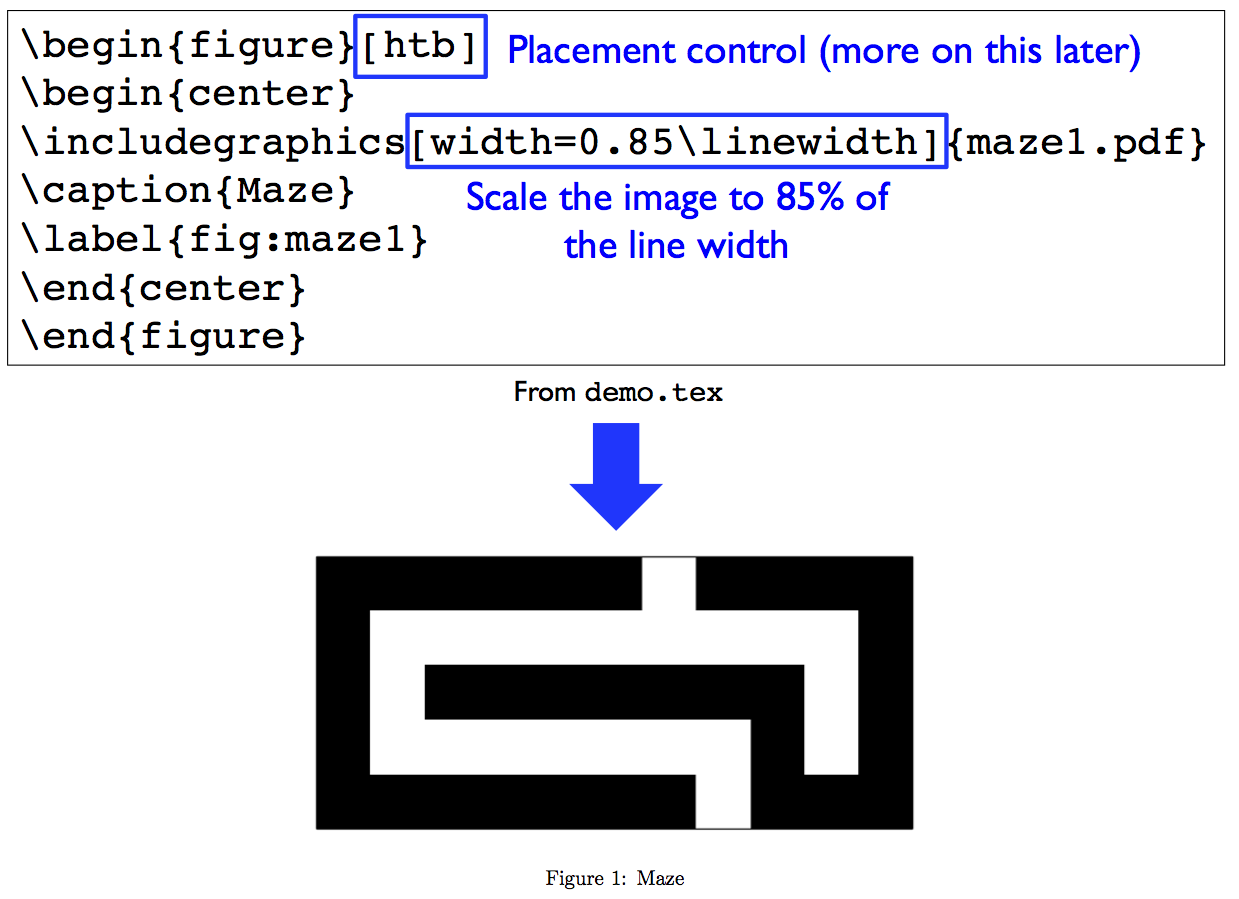
\includegraphics[scale=0.4]{fig/figure.png}
\caption{\footnotesize The
  \href{https://en.wikibooks.org/wiki/LaTeX/Floats,_Figures_and_Captions}
  {\emph{figure} environment} ensures that images
  aren't split across pages, and allows captions
  and references. The \texttt{$\backslash$center} environment ensures
  that we vertically align the figure on the page. We use the
  \texttt{$\backslash$includegraphics} command to import an actual
  image, where here we've specified to shrink the image
  somewhat. Lastly, the \texttt{$\backslash$label} command allows us
  to create a cross-reference for later use.}
\end{figure}

\newpage

\subsection{Tables}
\vspace{-2ex}
These can also be a bit overwhelming to learn at first, where similar
to our example on figures it may seem there are redundant commands used.
\begin{figure}[!h]
\centering
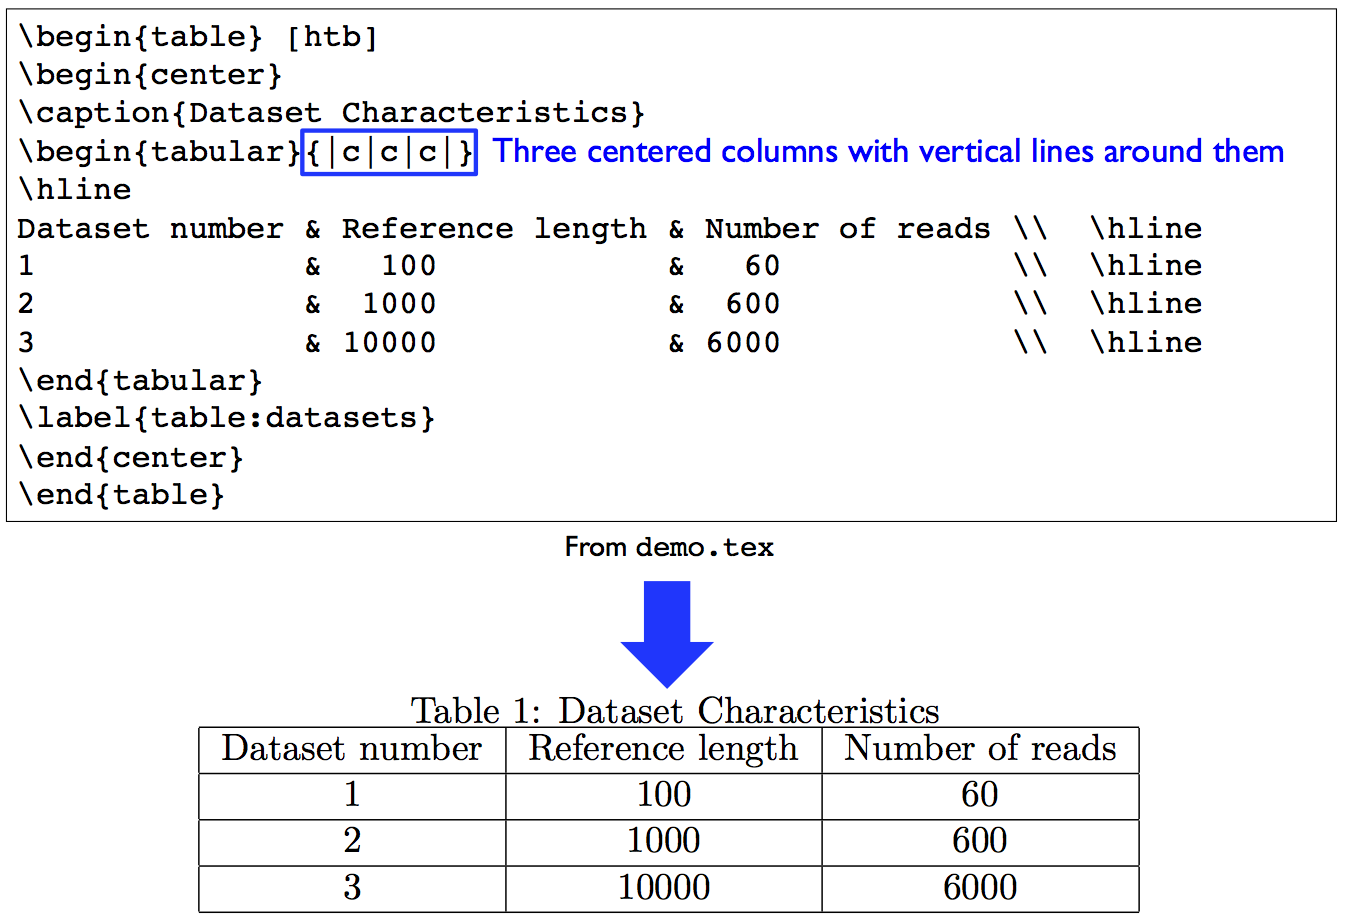
\includegraphics[scale=0.45]{fig/table.png}
\caption{\footnotesize
  The \texttt{table} environment declares a \texttt{float}ing
  object, i.e. one that cannot be split across pages. The \texttt{caption}
  command is effectively used as an input to our \texttt{table}
  environment. What's new here is the use of \texttt{tabular} to define
  a table environment. The required arguments for this environment are
  the number of columns in the table, and how they shall be aligned or
  delimited. I.e. we use one of \{\texttt{l,c,r}\} to denote left,
  central, or right alignment within a column; using a pipe character
  \texttt{|} signifies to delimit the columns by a vertical
  partitioner. In contrast to the number of columns (fixed by a required
  input argument to the \texttt{tabular} environment),
  the number of \emph{rows} is determined by the body of the
  environment. We use the \& character to delimit columns within a row,
  and two adjacent backslashes delimits the end of a row.}
\end{figure}

\subsubsection{Controlling Placement}

By default figures, tables, etc. will ``float'' around to where they
best fit. But, you can also specify preferences about placement.
Floating environments take a parameter in square brackets:
\texttt{\textbackslash{}begin\{figure\}{[}?{]}}. The options are:

\begin{itemize}
\item
  \texttt{h} for ``float here''
\item
  \texttt{t} for ``top of page''
\item
  \texttt{b} for ``bottom of page''
\item
  \texttt{H} for ``put here, don't float''
\end{itemize}
Good figure placement often requires some experimentation.
Advice: write the document first. Make it look nice second. Things
will change as you add more text and figures.

% \begin{figure}
% \centering
% 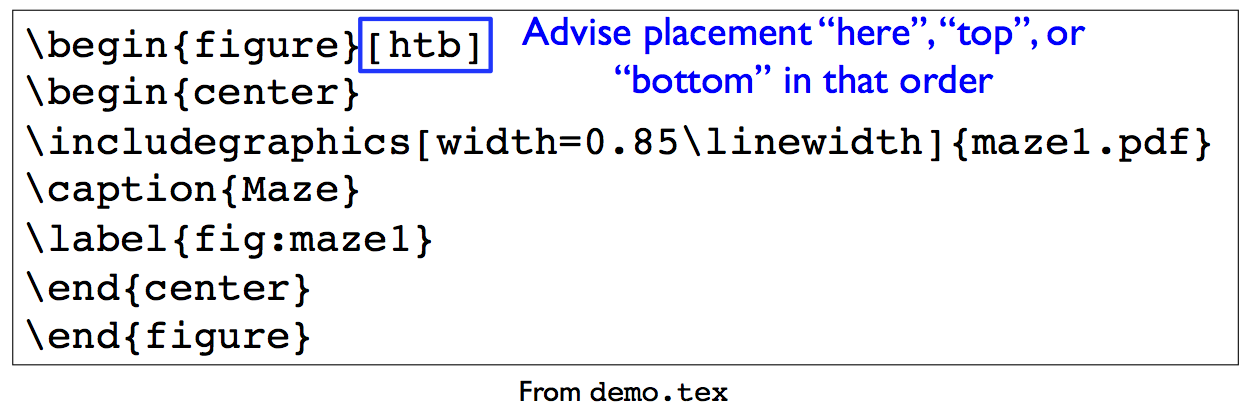
\includegraphics[scale=0.5]{fig/placement.png}
% \caption{fig}
% \end{figure}

\vspace{-2ex}
\subsection{Referencing Labels}
\label{sec: labels}
We may use
\texttt{\textbackslash{}label} and \texttt{\textbackslash{}ref}.

\begin{figure}[!h]
\centering
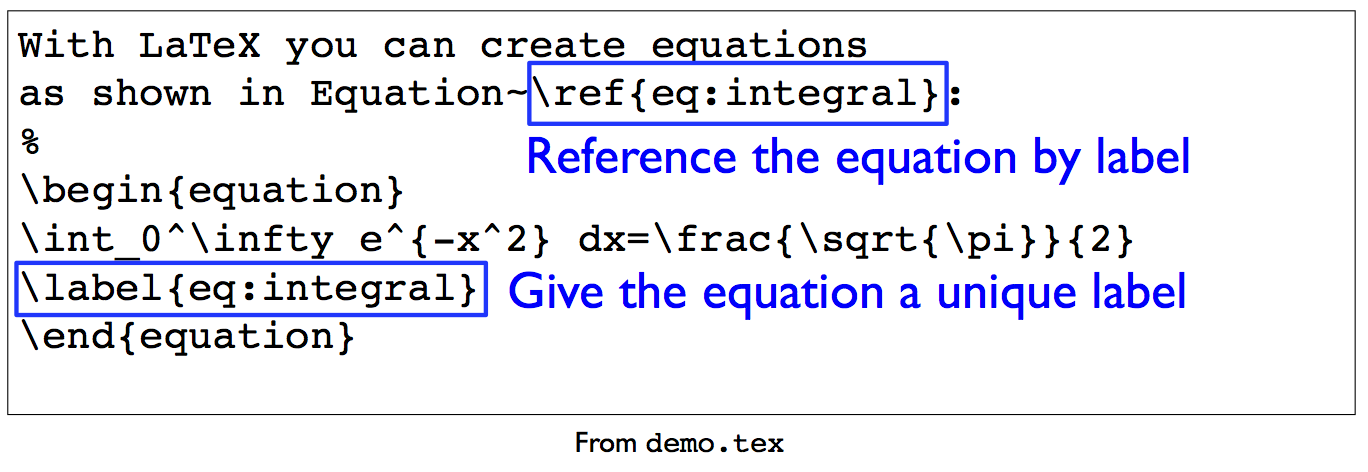
\includegraphics[scale=0.45]{fig/referencing.png}
\caption{\footnotesize
  Using a \texttt{ref} to mark a point of interest, and
  \texttt{label} to cite it. One great advantage here when compared
  with conventional word processors is that all of our linking is done
  dynamically. E.g. if we choose, we can use a table of contents or
  table of figures, and the page-numbering and table/figure numbers
  will be automatically updated whenever we update the document. This
  can save against some nasty errors wherein we may insert a new
  figure into the body of our document but forget to update the table
  of contents.}
\end{figure}

The first pass of LaTeX will produce an unresolved reference:
\begin{figure}[h]
\centering
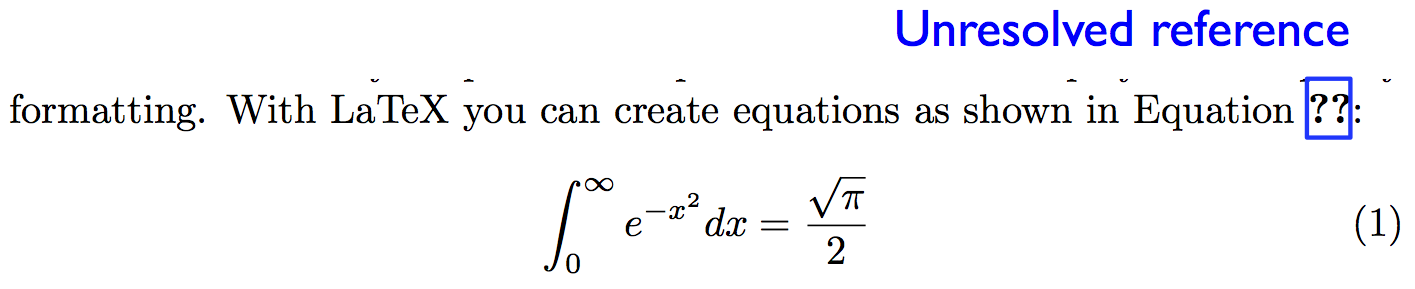
\includegraphics[scale=0.4]{fig/unresolved-reference.png}
\caption{An example of what an unresolved reference looks like within
  a rendered \TeX \, document.}
\end{figure}

The second pass of LaTeX will actually resolve the reference.

\begin{figure}[h]
\centering
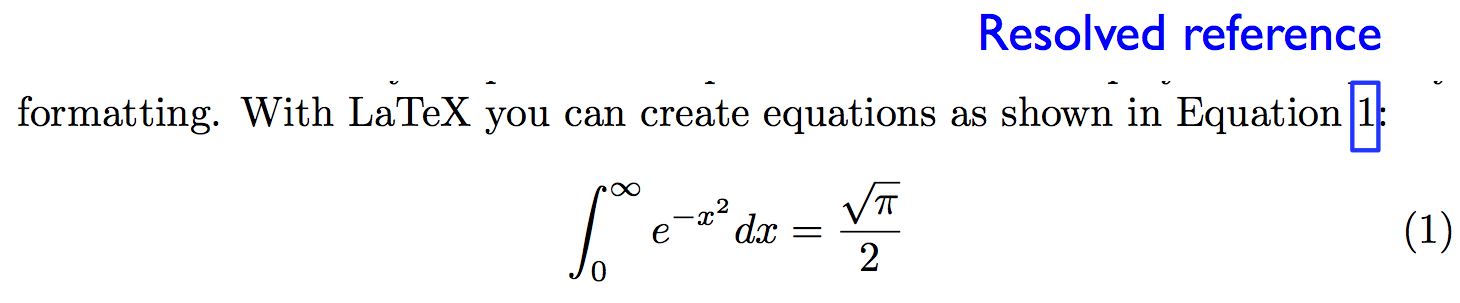
\includegraphics[scale=0.4]{fig/resolved-reference.png}
\caption{An example of what the corresponding resolved reference might
look like in our rendered example.}
\end{figure}

\subsection{Algorithms}
Another fantastic use of \TeX \, is in describing sub-routines and
algorithms. I preference the \texttt{algorithm2e} package; it is
quite flexible and formats nicely.

\begin{figure}[!h]
\centering
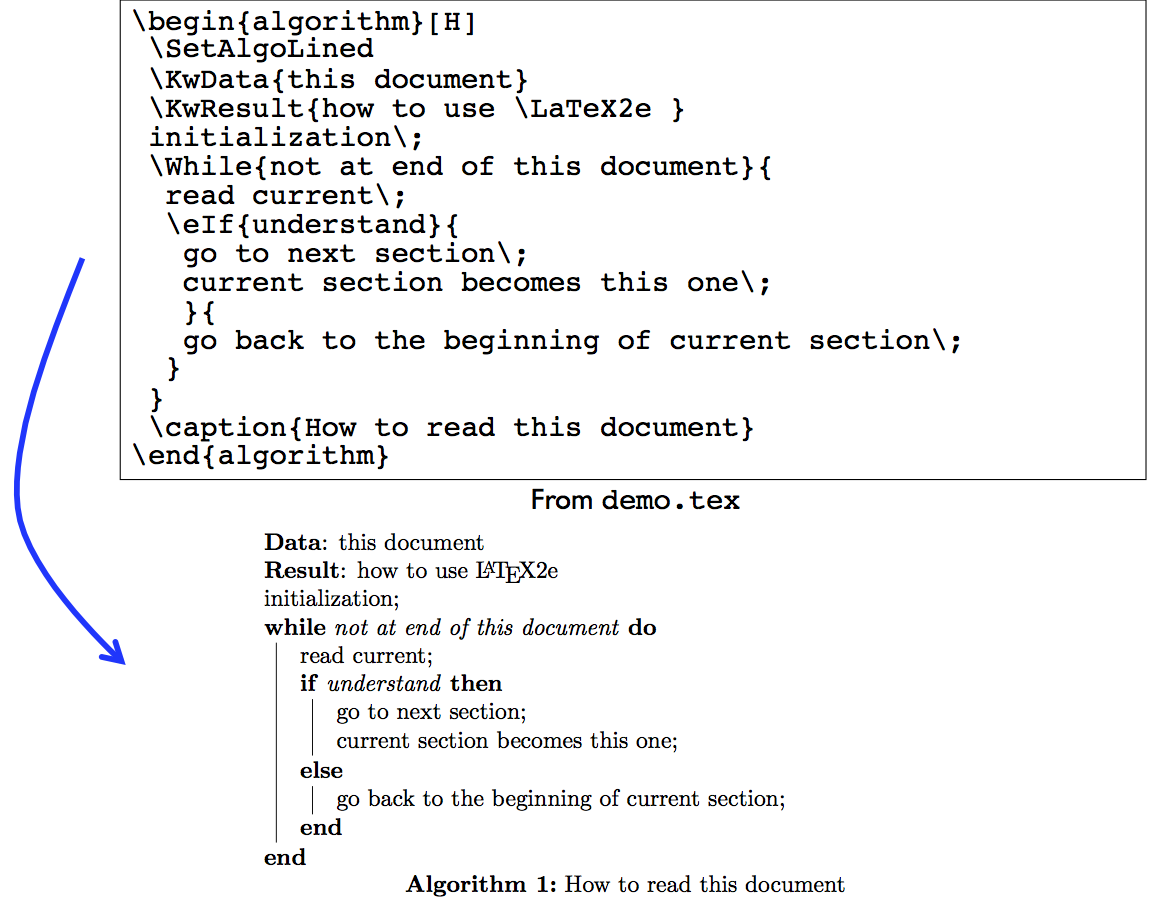
\includegraphics[scale=0.5]{fig/algorithm.png}
\caption{\footnotesize
  An example of the \texttt{algorithm} environment provided by
  \texttt{alborithm2e} package. Notice that we can declare our input
  data and output results, which are essential for those unfamiliar
  with the sub-routine to understand its high-level purpose. We also
  have access to control-flow structures, and we can use all of our
  usual \TeX \, symbols or mathematical formatting.
  Not featured in the above example: I like to use
  \texttt{$\backslash$tcp\{comment\}} to include inline comments using
  the C++ style of \texttt{//}.
}
\end{figure}
\section{Bibliographies}
\subsection{BibTex}
This is a companion program for managing citations of
papers, books, websites, etc.
We start by creating a \texttt{.bib} file.
E.g. see \texttt{tex/references.bib}:

\begin{figure}[h]
\centering
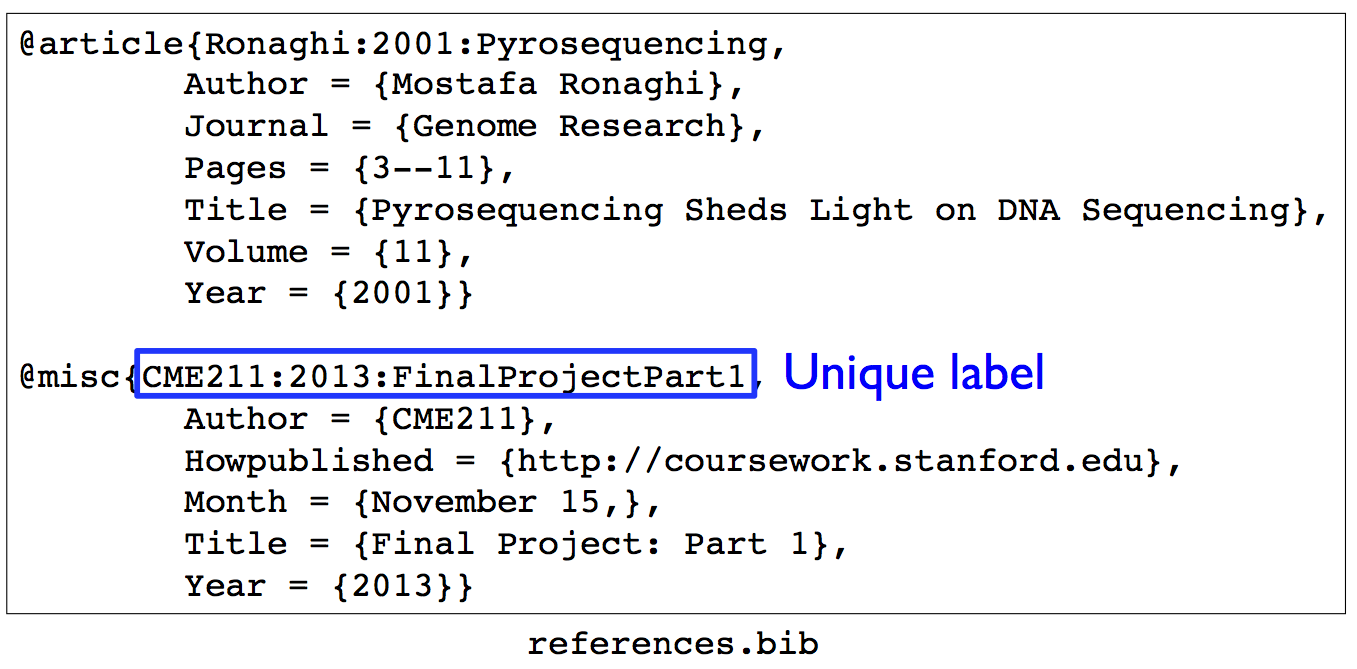
\includegraphics[scale=0.4]{fig/bibtex-example.png}
\caption{\footnotesize We demonstrate the formatting of a
  \href{http://www.bibtex.org/Using/}{\texttt{.bib}} file. For more
  details, see the \href{http://www.bibtex.org/Format/}{BibTex format specs}.}
\end{figure}

\vspace{-2ex}
\subsection{Citations}
Citations in \LaTeX \, simply use the \texttt{cite} command, where the
argument specifies which entry in the BibTex file to use.

\begin{figure}[!h]
\centering
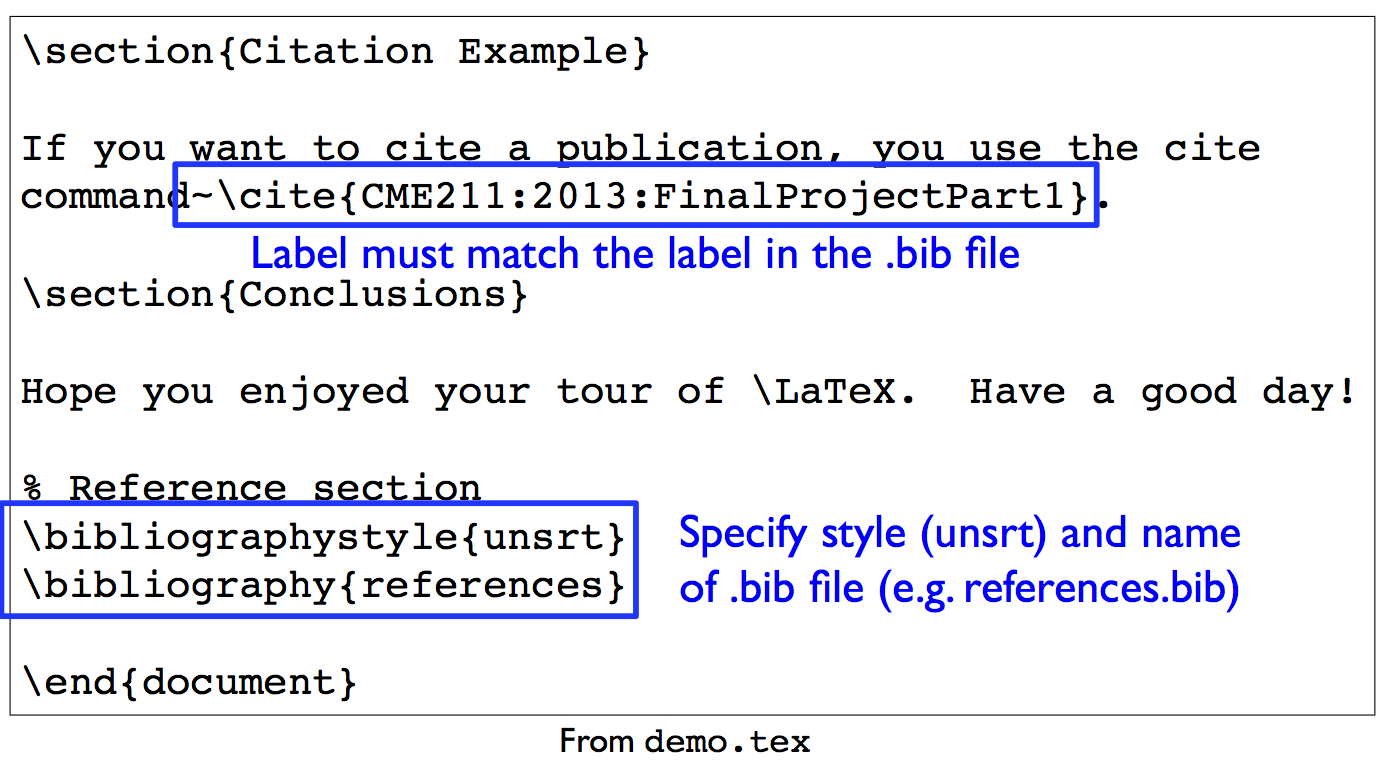
\includegraphics[scale=0.425]{fig/citations.png}
\caption{\footnotesize
  We use \texttt{cite} to indicate a reference toward a
  bibliographic citation. This is different from referencing a labeled
object, described earlier in section \ref{sec: labels}!}
\end{figure}

Resulting PDF:

\begin{figure}[!h]
\centering
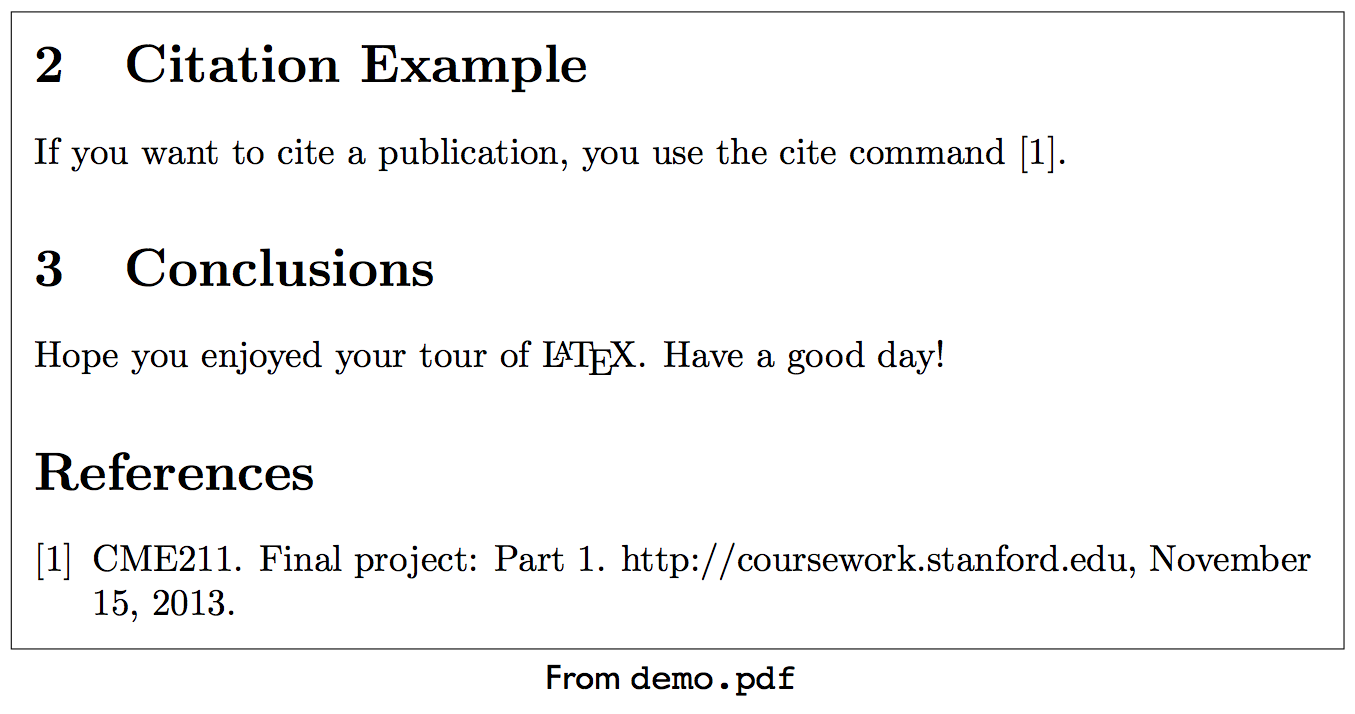
\includegraphics[scale=0.375]{fig/demo-pdf.png}
\caption{\footnotesize
  We emphasize that the references are dynamic. Want to switch
 to lexicographic ordering of listings in the bibliography? No need to
switch all of our citations, simply update the bibliography style in a
single place! Re-compiling our document (a couple times) will yield
updated references.}
\end{figure}

\paragraph{Typesetting with BibTeX Reference}
This can be annoying at first! In order to get
references correct, we
\href{https://tex.stackexchange.com/a/53236/48589}{must take a couple
  passes}
through the document.

{\footnotesize
\begin{verbatim}
$ pdflatex demo     # Take args to \cite, write to .aux file.
$ bibtex demo       # Formats these according to user-specs, write to .bbl file.
$ pdflatex demo     # Inserts the .bbl file into .tex file at point of \bibliography.
                    # Correct labels for \cite commands written in .aux file.
$ pdflatex demo     # Only now does LaTeX know what correct labels to include in doc.
\end{verbatim}
}

Although any text editor can be used to create, edit, and manage a
\texttt{.bib} file,
some editors will recognize the file extension and enable a BibTex
specific mode.
There are also applications \emph{specifically} for doing this:
\href{http://bibdesk.sourceforge.net}{BibDesk} (MacOSx only),
\href{http://jabref.sourceforge.net}{Jabref} (any OS), and
\href{http://www.mendeley.com}{Mendeley}.

\vspace{-2ex}
\section{A note on LaTeX errors}

LaTeX will dump error messages and start a prompt on errors:
{\footnotesize
\begin{verbatim}
$ pwd
/Users/nwh/Dropbox/courses/2015-Q4-cme211/lecture-prep/lecture-13-work/tex
nwh-mbpro:tex nwh$ pdflatex demo
This is pdfTeX, Version 3.14159265-2.6-1.40.16 (TeX Live 2015) (preloaded format=pdflatex)
.....
) (./demo.aux) (/usr/local/texlive/2015/texmf-dist/tex/latex/base/omscmr.fd)
! Undefined control sequence.
l.35 \includegraphics[scale=0.5]
                     [width=0.85\linewidth]{../fig/maze.pdf}
? 
\end{verbatim}
}

LaTeX is prompting you how to continue. See \LaTeX \,
\href{https://en.wikibooks.org/wiki/LaTeX/Errors_and_Warnings#Error_messages}{errors
  and warnings}. We may type \texttt{x} to e\textbf{x}it the program,
\texttt{q} to \textbf{q}uietly carry on with execution, or for example
\texttt{h} for more \textbf{h}elp.
In our example, we could type \texttt{x} to quit the compilation
process, then fix the error in the \texttt{.tex} file and try again.
In this case, we
forgot \texttt{\textbackslash{}usepackage\{graphicx\}} in the preamble.

\textbf{References:} Apart from Google,
{
  \small
\begin{itemize}
\item
  Guide to LaTeX by Kopka and Daly:\\
  \url{http://proquest.safaribooksonline.com/book/graphic-design/9780321617736}
\item
  \textbf{Detexify}: a web tool to go from symbol drawing to TeX
  command:\\
  \url{http://detexify.kirelabs.org/classify.html}
\item
  LaTeX Wikibook: \url{https://en.wikibooks.org/wiki/LaTeX}
\item A Gentle Introduction to \TeX:
  \footnotesize \url{http://texdoc.net/texmf-dist/doc/plain/gentle/gentle.pdf}
\item How to draw in \TeX: \url{http://www.texample.net/tikz/}
\end{itemize}
}

\end{document}